\documentclass[specialist, subf, href, colorlinks=true, 14pt, times, mtpro, final]{disser}

\usepackage[english, russian]{babel}
\usepackage[T2A]{fontenc}
\usepackage [utf8] {inputenc}
\usepackage{amsmath,amsthm,amssymb}
\usepackage {wrapfig}
\usepackage {enumitem}  
\usepackage{graphicx}
\usepackage{multicol}
\usepackage{mathrsfs}
\usepackage{xcolor}
\usepackage{hyperref}
\usepackage{tikz}
\usepackage{pdfpages}


\usetikzlibrary{decorations.pathreplacing}
\usepackage[noend]{algpseudocode}
\usepackage[a4paper, mag=1000, includefoot, left=3cm, right=1.5cm, top=2cm, bottom=2cm, headsep=1cm, footskip=1cm]{geometry}
\usepackage{floatrow}
\usepackage{tikz}
\usetikzlibrary{graphs}

\theoremstyle{definition}
\newtheorem{defn}{Определение}[section]
\newtheorem{example}{Пример}[section]
\newtheorem{state}{Утверждение}[section]
\newtheorem{theorem}{Теорема}[section]
\newtheorem{lemma}{Лемма}[section]
\newtheorem{axiom}{Аксиома}[section]
\newtheorem{consequence}{Следствие}[section]

\begin{document}
	\begin{titlepage}
	\begin{center}

		Федеральное государственное бюджетное образовательное учреждение высшего образования 
		<<Московский Государственный Университет им.\,М.\,В.\,Ломоносова>>\\
		
		Механико-математический факультет
		
		Кафедра вычислительной математики\\[0.6cm]
		
		\begin{figure}[!htp]
				\begin{center}
						{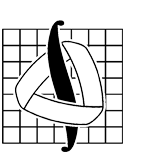
\includegraphics[width=20mm]{pics/mmlogo.png}}
					\end{center}
			\end{figure}
		
		\vspace{3cm}
			
		{\bf Численное моделирование нестационарного одномерного течения газа с использованием неявной параллельной разностной схемой с центральными разностями $(\rho, u)$}
		
		\vspace{5cm}
		\begin{flushright}
			{\bfРаботу выполнил:}\\
			студент 4 курса Сибгатуллин Артур Петрович\\[0.5cm]
		\end{flushright}
		\vspace{1cm}
		
		\normalsize Москва, 2021
	\end{center}
\end{titlepage}

	
	\tableofcontents
	\newpage
	
	\section{Введение}
\subsection{Постановка задачи}

Рассмотрим систему уравнений, описывающую нестационарное одномерное движение вязкого баротропного газа:

\begin{equation} \label{eq:task}
	\begin{cases}
		\begin{array}{l}
			\frac{\partial\rho}{\partial t} + \frac{\partial \rho u}{\partial x} = \rho f_0 \\
			\rho \frac{\partial u}{\partial t} + \rho u \frac{\partial u}{\partial x} + \frac{\partial p}{\partial x} = \mu \frac{\partial^2u}{\partial x^2} + \rho \\
			p = p(\rho)
		\end{array}
	\end{cases}
\end{equation}

Через $\mu$ обозначен коэффициент вязкости газа, который будем считать известной положительной
константой. Известными также будем считать функцию давления газа $p$ (в данной работе будем рассматривать $p(\rho) = C\rho$, где $C$ - положительная константа) и вектор внешних сил $f$. $f$ - функция переменных Эйлера: $(t, \, x) \in Q = \Omega_t \times \Omega_x = [0; \, T] \times [0; \, X]$.

Неизвестные функции: плотность $\rho$ и скорость $u$ также являются функциями переменных Эйлера.

Перепишем систему $(1)$ в эквивалентный вид, при условии того, что $\rho$ и $u$ гладкие: 

\begin{equation} \label{eq:task_reformulate}
	\begin{cases}
		\begin{array}{l}
			\frac{\partial \rho}{\partial t} + \frac{1}{2}\left(u\frac{\partial \rho}{\partial x} + \frac{\partial \rho u}{\partial x} + \rho \frac{\partial u}{\partial x}\right) = 0\\
			\frac{\partial u}{\partial t} + \frac{1}{3}\left(u\frac{\partial u}{\partial x} + \frac{\partial u^2}{\partial x}\right) +\frac{1}{\rho}\frac{\partial p}{\partial x} = \frac{\mu}{\rho}\frac{\partial^2 u}{\partial x^2} + f			
		\end{array}
	\end{cases}
\end{equation}

Система \eqref{eq:task} дополнена граничными условиями:
\begin{equation} \label{eq:terms}
	\begin{array}{lc}
		(\rho, \, u)|_{t = 0} = (\rho_0, \, u_0), &\quad x \in [0; \, X] \\
		u (t, \, 0) = u (t, \, X) = 0, &\quad t \in [0; \, T]
	\end{array}
\end{equation}

\subsection{Основные обозначения}
Введем на $\Omega_x$ и $\Omega_t$ сетки:
\begin{equation}
	\begin{array}{lc}
		\omega_x = \{mh: m = 0, \dots, M\}, h = \frac{X}{M}\\
		\omega_t = \{n\tau: n = 0, \dots, N\}, \tau = \frac{T}{N}\\
	\end{array}
\end{equation}

Для сокращения записи значение для произвольной функции f в узле $(n,m)$ сетки $\omega_x x \omega_t$ обозначим за $f_m^n$. Введем следующие обозначения:
\begin{equation}
	\begin{array}{lc}
		\hat{f} = f_m^{n+1}\\
		f_t = \frac{f_m^{n+1} - f_m^n}{\tau}\\
		f_x = \frac{f_{m+1}^n - f^n_m}{h}\\
		f_{\bar{x}} = \frac{f_m^n - f^n_{m-1}}{h}\\
		f_{\mathring{x}} = \frac{f_{m+1}^n - f^n_{m-1}}{2h}\\
		f_{x\bar{x}} = \frac{f^n_{m-1} - 2f_m^n + f^n_{m+1}}{h^2}\\
	\end{array}
\end{equation}
	
	
	\newpage
\section{Разностная схема}
\subsection{Описание схемы}

Для поиска численного решения задачи $(1)$ можно использовать разностную схему, в которой при апроксимации конвективных членов используются центральные разности, а приближенные значения плотности $H$ и скорости $V$ на каждом временном слое ищутся в узлах сетки $\Omega_h$ как решения двух СЛАУ, порядок решения которых произволен:

$$H_t + 0.5\sum_{k=1}^2(V_k\hat{H}_{\mathring{x}_k} + (V_k\hat{H})_{\mathring{x}_k} + H(V_k)_{\mathring{x}_k}) = 0, w \in \Omega_h \eqno(2.1)$$

$$H_t + 0.5((V_k\hat{H})_{x_k} + H(V_k)_{x_k}) - 0.5h_k((HV_k)_{x_k\bar{x}_k}^{+1_k} - 0.5(HV_k)_{x_k\bar{x}_k}^{+2_k} + $$
$$+ H((V_k)_{x_k\bar{x}_k}^{^+1_k} - 0.5(V_k)_{x_k\bar{x}_k}^{+2_k})) = 0, x \in \gamma_k^-  \eqno(2.2)$$

$$H_t + 0.5((V_k\hat{H})_{\bar{x}_k} + H(V_k)_{\bar{x}_k}) - 0.5h_k((HV_k)_{x_k\bar{x}_k}^{-1_k} - 0.5(HV_k)_{x_k\bar{x}_k}^{-2_k} + $$
$$ + H((V_k)_{x_k\bar{x}_k}^{^-1_k} - 0.5(V_k)_{x_k\bar{x}_k}^{-2_k})) = 0, x \in \gamma_k^-  \eqno(2.3)$$

$$(V_k)_t + \frac{1}{3}(V_k(\hat{V}_k)_{\mathring{x}_k} + (V_k\hat{V}_k)_{\mathring{x}_k}) + $$
$$\frac{1}{2}\sum_{m=1, m\neq k}^2 \left(V_m(\hat{V}_k)_{\mathring{x}_m} + (V_m\hat{V}_k)_{\mathring{x}_m} - V_k(V_m)_{\mathring{x}_m} \right) + \frac{p(H)_{\mathring{x}_k}}{H} = $$
$$ = \tilde{\mu}\left(\frac{4}{3}(\hat{V}_k)_{x_k\bar{x}_k} + \sum_{m=1, m\neq k}^{2} (\hat{V}_k)_{x_m\bar{x}_m}\right) - (\tilde{\mu} - \frac{\mu}{H})\left(\frac{4}{3}(V_k)_{x_k\bar{x}_k} + \sum_{m=1, m\neq k}^{2} (V_k)_{x_m\bar{x}_m}\right) + $$
$$ + \frac{\mu}{3H}\sum_{m=1, m\neq k}^{2}(V_m)_{\mathring{x}_k\mathring{x}_m} + f_k, x\in \Omega_h  \eqno(2.4)$$

$$\hat{V}_k = 0, x \in \gamma_{h}^-, k=1,2  \eqno(2.5)$$

Где:
$$\tilde{\mu} = \max_m \frac{\mu}{H}$$

\subsection{Координатная запись}
Распишем схему приведенных выше обозначениях, и выделим коэффиценты при $H\,$ и $V$ на $n + 1$ временном слое:
\subsubsection{1 уравнение (2.1)}
$$H_t + 0.5\sum_{k=1}^2(V_k\hat{H}_{\mathring{x}_k} + (V_k\hat{H})_{\mathring{x}_k} + H(V_k)_{\mathring{x}_k}) = 0$$\\

$
2\frac{H^{n+1}_{m_1, m_2} - H^n_{m_1, m_2}}{\tau} + V_{1 \, m_1, m_2}^n \frac{H_{m_1 + 1, m_2}^{n+1} - H_{m_1 - 1, m_2}^{n+1}}{2h_1} + \frac{V_{1 \, m_1+1, m_2}^nH_{m_1+1, m_2}^{n+1} - V_{1 \, m_1-1, m_2}^nH_{m_1-1, m_2}^{n+1}}{2h_1} + \\
+ H_{m_1, m_2}^n\left(\frac{V_{1 \, m_1 + 1, m_2}^n - V_{1 \, m_1 - 1, m_2}^n}{2h_1}\right) + \\
+ V_{2 \, m_1, m_2}^n \frac{H_{m_1, m_2 + 1}^{n+1} - H_{m_1, m_2 - 1}^{n+1}}{2h_2} + \frac{V_{2 \, m_1, m_2+1}^nH_{m_1, m_2+1}^{n+1} - V_{2 \, m_1, m_2-1}^nH_{m_1, m_2 - 1}^{n+1}}{2h_2} + \\
+ H_{m_1, m_2}^n\left(\frac{V_{2 \, m_1, m_2 + 1}^n - V_{2 \, m_1, m_2 - 1}^n}{2h_2}\right) = 0
$\\

$
H_{m_1 - 1, m_2}^{n+1} (-\frac{V_{1 \, m_1, m_2}^n + V_{1 \, m_1 - 1, m_2}^n}{2h_1}) + H_{m_1, m_2}^{n+1}(\frac{2}{\tau}) + H_{m_1 + 1, m_2}^{n+1}(\frac{V_{1 \, m_1, m_2}^n + V_{1 \, m_1 + 1, m_2}^n}{2h_1}) + \\
+ H_{m_1, m_2 - 1}^{n+1} (-\frac{V_{2 \, m_1, m_2}^n + V_{2 \, m_1, m_2 - 1}^n}{2h_2}) + H_{m_1, m_2}^{n+1}(0) + H_{m_1, m_2 + 1}^{n+1}(\frac{V_{2 \, m_1, m_2}^n + V_{1 \, m_1, m_2 + 1}^n}{2h_2}) = \\
= -\frac{2H_{m_1, m_2}^n}{\tau} - H_{m_1, m_2}^n \left(\frac{V_{1 \, m_1 + 1, m_2}^n - V_{1 \, m_1 - 1, m_2}^n}{2h_1} + \frac{V_{2 \, m_1, m_2 + 1}^n - V_{2 \, m_1, m_2 - 1}^n}{2h_2}\right)
$\\

\newpage
\subsubsection{2 уравнение (2.2)}
$$H_t + 0.5((V_k\hat{H})_{x_k} + H(V_k)_{x_k}) - 0.5h_k((HV_k)_{x_k\bar{x}_k}^{+1_k} - 0.5(HV_k)_{x_k\bar{x}_k}^{+2_k} + $$
$$+ H((V_k)_{x_k\bar{x}_k}^{^+1_k} - 0.5(V_k)_{x_k\bar{x}_k}^{+2_k})) = 0$$\\

Распишем случай для $k = 1$:
$$H_t + 0.5((V_1\hat{H})_{x_1} + H(V_1)_{x_1}) - 0.5h_1((HV_1)_{x_1\bar{x}_1}^{+1_1} - 0.5(HV_1)_{x_1\bar{x}_1}^{+2_1} + $$
$$+ H((V_1)_{x_1\bar{x}_1}^{^+1_1} - 0.5(V_1)_{x_1\bar{x}_1}^{+2_1})) = 0$$\\

$
\frac{H^{n+1}_{m_1, m_2} - H^n_{m_1, m_2}}{\tau} + 0.5(\frac{V_{1 \, m_1 + 1, m_2}^nH_{m_1 + 1, m_2}^{n+1} - V_{1 \, m_1, m_2}^nH_{m_1, m_2}^{n+1}}{h_1} + H_{m_1, m_2}^n\frac{V_{1 \, m_1 + 1, m_2}^n - V_{1 \, m_1, m_2}^n}{h_1}) - \\
- 0.5h_1((\frac{H_{m_1, m_2}^nV_{1 \, m_1, m_2}^n - 2H_{m_1 + 1, m_2}^nV_{1 \, m_1 + 1, m_2}^n + H_{m_1+2, m_2}^nV_{1 \, m_1+2, m_2}^n}{h_1^2}) - \\
- 0.5\frac{H_{m_1+1, m_2}^nV_{1 \, m_1+1, m_2}^n - 2H_{m_1 + 2, m_2}^nV_{1 \, m_1 + 2, m_2}^n + H_{m_1+3, m_2}^nV_{1 \, m_1+3, m_2}^n}{h_1^2} + \\
+ H_{m_1, m_2}^n(\frac{V_{1 \, m_1, m_2}^n - 2V_{1 \, m_1 + 1, m_2}^n + V_{1 \, m_1+2, m_2}^n}{h_1^2} - 0.5\frac{V_{1 \, m_1 + 1, m_2}^n - 2V_{1 \, m_1 + 2, m_2}^n + V_{1 \, m_1+3, m_2}^n}{h_1^2})) = 0
$\\

$
H_{m_1 - 1, m_2}^{n+1} (0) + H_{m_1, m_2}^{n+1}(\frac{1}{\tau} - 0.5\frac{V_{1 \, m_1, m_2}^n}{h_1}) + H_{m_1 + 1, m_2}^{n+1}(0.5\frac{V_{1 \, m_1 + 1, m_2}^n}{h_1}) + \\
+ H_{m_1, m_2 - 1}^{n+1} (0) + H_{m_1, m_2}^{n+1}(0) + H_{m_1, m_2 + 1}^{n+1}(0) =\\
= -0.5H_{m_1, m_2}^n\frac{V_{1 \, m_1+1, m_2}^n - V_{1 \, m_1, m_2}^n}{h_1} + \frac{H_{m_1, m_2}^n}{\tau} +\\
+ 0.5h_1((\frac{H_{m_1, m_2}^nV_{1 \, m_1, m_2}^n - 2H_{m_1 + 1, m_2}^nV_{1 \, m_1 + 1, m_2}^n + H_{m_1+2, m_2}^nV_{1 \, m_1+2, m_2}^n}{h_1^2}) - \\
- 0.5\frac{H_{m_1+1, m_2}^nV_{1 \, m_1+1, m_2}^n - 2H_{m_1 + 2, m_2}^nV_{1 \, m_1 + 2, m_2}^n + H_{m_1+3, m_2}^nV_{1 \, m_1+3, m_2}^n}{h_1^2} + \\
+ H_{m_1, m_2}^n(\frac{V_{1 \, m_1, m_2}^n - 2V_{1 \, m_1 + 1, m_2}^n + V_{1 \, m_1+2, m_2}^n}{h_1^2} - 0.5\frac{V_{1 \, m_1 + 1, m_2}^n - 2V_{1 \, m_1 + 2, m_2}^n + V_{1 \, m_1+3, m_2}^n}{h_1^2}))
$\\

\newpage
Распишем случай для $k = 2$:
$$H_t + 0.5((V_2\hat{H})_{x_2} + H(V_2)_{x_2}) - 0.5h_2((HV_2)_{x_2\bar{x}_2}^{+1_2} - 0.5(HV_2)_{x_2\bar{x}_2}^{+2_2} + $$
$$+ H((V_2)_{x_2\bar{x}_2}^{^+1_2} - 0.5(V_2)_{x_2\bar{x}_2}^{+2_2})) = 0$$\\

$
\frac{H^{n+1}_{m_1, m_2} - H^n_{m_1, m_2}}{\tau} + 0.5(\frac{V_{2 \, m_1, m_2+1}^nH_{m_1, m_2+1}^{n+1} - V_{2 \, m_1, m_2}^nH_{m_1, m_2}^{n+1}}{h_2} + H_{m_1, m_2}^n\frac{V_{2 \, m_1, m_2+1}^n - V_{2 \, m_1, m_2}^n}{h_2}) - \\
- 0.5h_2((\frac{H_{m_1, m_2}^nV_{2 \, m_1, m_2}^n - 2H_{m_1, m_2 + 1}^nV_{2 \, m_1, m_2 + 1}^n + H_{m_1, m_2+2}^nV_{2 \, m_1, m_2+2}^n}{h_2^2}) - \\
- 0.5\frac{H_{m_1, m_2+1}^nV_{2 \, m_1, m_2+1}^n - 2H_{m_1, m_2 + 2}^nV_{2 \, m_1, m_2 + 2}^n + H_{m_1, m_2+3}^nV_{2 \, m_1, m_2+3}^n}{h_2^2} + \\
+ H_{m_1, m_2}^n(\frac{V_{2 \, m_1, m_2}^n - 2V_{2 \, m_1, m_2+1}^n + V_{2 \, m_1, m_2+2}^n}{h_2^2} - 0.5\frac{V_{2 \, m_1, m_2+1}^n - 2V_{2 \, m_1, m_2+2}^n + V_{2 \, m_1, m_2+3}^n}{h_2^2})) = 0
$\\

$
H_{m_1 - 1, m_2}^{n+1} (0) + H_{m_1, m_2}^{n+1}(0) + H_{m_1 + 1, m_2}^{n+1}(0) + \\
+ H_{m_1, m_2 - 1}^{n+1} (0) + H_{m_1, m_2}^{n+1}(\frac{1}{\tau} - 0.5\frac{V_{2 \, m_1, m_2}^n}{h_2}) + H_{m_1, m_2 + 1}^{n+1}(0.5\frac{V_{2 \, m_1, m_2+1}^n}{h_2}) =\\
= -0.5H_{m_1, m_2}^n\frac{V_{2 \, m_1, m_2+1}^n - V_{2 \, m_1, m_2}^n}{h_2} + \frac{H_{m_1, m_2}^n}{\tau} +\\
+ 0.5h_2((\frac{H_{m_1, m_2}^nV_{2 \, m_1, m_2}^n - 2H_{m_1, m_2+1}^nV_{2 \, m_1, m_2+1}^n + H_{m_1, m_2+2}^nV_{2 \, m_1, m_2+2}^n}{h_2^2}) - \\
- 0.5\frac{H_{m_1, m_2+1}^nV_{2 \, m_1, m_2+1}^n - 2H_{m_1, m_2+2}^nV_{2 \, m_1, m_2+2}^n + H_{m_1, m_2+3}^nV_{2 \, m_1, m_2+3}^n}{h_2^2} + \\
+ H_{m_1, m_2}^n(\frac{V_{2 \, m_1, m_2}^n - 2V_{2 \, m_1, m_2+1}^n + V_{2 \, m_1, m_2+2}^n}{h_2^2} - 0.5\frac{V_{2 \, m_1, m_2+1}^n - 2V_{2 \, m_1, m_2+2}^n + V_{2 \, m_1, m_2+3}^n}{h_2^2}))
$

\newpage
\subsubsection{3 уравнение (2.3)}
$$H_t + 0.5((V_k\hat{H})_{\bar{x}_k} + H(V_k)_{\bar{x}_k}) - 0.5h_k((HV_k)_{x_k\bar{x}_k}^{-1_k} - 0.5(HV_k)_{x_k\bar{x}_k}^{-2_k} + $$
$$ + H((V_k)_{x_k\bar{x}_k}^{^-1_k} - 0.5(V_k)_{x_k\bar{x}_k}^{-2_k})) = 0$$\\

Распишем случай для $k = 1$:
$$H_t + 0.5((V_1\hat{H})_{\bar{x}_1} + H(V_1)_{\bar{x}_1}) - 0.5h_1((HV_1)_{x_1\bar{x}_1}^{-1_1} - 0.5(HV_1)_{x_1\bar{x}_1}^{-2_1} + $$
$$+ H((V_1)_{x_1\bar{x}_1}^{^-1_1} - 0.5(V_1)_{x_1\bar{x}_1}^{-2_1})) = 0$$\\

$
\frac{H^{n+1}_{m_1, m_2} - H^n_{m_1, m_2}}{\tau} + 0.5(\frac{V_{1 \, m_1, m_2}^nH_{m_1, m_2}^{n+1} - V_{1 \, m_1-1, m_2}^nH_{m_1-1, m_2}^{n+1}}{h_1} + H_{m_1, m_2}^n\frac{V_{1 \, m_1, m_2}^n - V_{1 \, m_1-1, m_2}^n}{h_1}) - \\
- 0.5h_1((\frac{H_{m_1-2, m_2}^nV_{1 \, m_1-2, m_2}^n - 2H_{m_1-1, m_2}^nV_{1 \, m_1-1, m_2}^n + H_{m_1, m_2}^nV_{1 \, m_1, m_2}^n}{h_1^2}) - \\
- 0.5\frac{H_{m_1-3, m_2}^nV_{1 \, m_1-3, m_2}^n - 2H_{m_1-2, m_2}^nV_{1 \, m_1-2, m_2}^n + H_{m_1-1, m_2}^nV_{1 \, m_1-1, m_2}^n}{h_1^2} + \\
+ H_{m_1, m_2}^n(\frac{V_{1 \, m_1-2, m_2}^n - 2V_{1 \, m_1-1, m_2}^n + V_{1 \, m_1, m_2}^n}{h_1^2} - 0.5\frac{V_{1 \, m_1-3, m_2}^n - 2V_{1 \, m_1-2, m_2}^n + V_{1 \, m_1-1, m_2}^n}{h_1^2})) = 0
$\\

$
H_{m_1 - 1, m_2}^{n+1} (-0.5\frac{V_{1 \, m_1-1, m_2}^n}{h_1}) + H_{m_1, m_2}^{n+1}(\frac{1}{\tau} + 0.5\frac{V_{1 \, m_1, m_2}^n}{h_1}) + H_{m_1 + 1, m_2}^{n+1}(0) + \\
+ H_{m_1, m_2 - 1}^{n+1} (0) + H_{m_1, m_2}^{n+1}(0) + H_{m_1, m_2 + 1}^{n+1}(0) =\\
= -0.5H_{m_1, m_2}^n\frac{V_{1 \, m_1, m_2}^n - V_{1 \, m_1-1, m_2}^n}{h_1} + \frac{H_{m_1, m_2}^n}{\tau} +\\
+ 0.5h_1((\frac{H_{m_1-2, m_2}^nV_{1 \, m_1-2, m_2}^n - 2H_{m_1-1, m_2}^nV_{1 \, m_1-1, m_2}^n + H_{m_1, m_2}^nV_{1 \, m_1, m_2}^n}{h_1^2}) - \\
- 0.5\frac{H_{m_1-3, m_2}^nV_{1 \, m_1-3, m_2}^n - 2H_{m_1-2, m_2}^nV_{1 \, m_1-2, m_2}^n + H_{m_1-1, m_2}^nV_{1 \, m_1-1, m_2}^n}{h_1^2} + \\
+ H_{m_1, m_2}^n(\frac{V_{1 \, m_1-2, m_2}^n - 2V_{1 \, m_1-1, m_2}^n + V_{1 \, m_1, m_2}^n}{h_1^2} - 0.5\frac{V_{1 \, m_1-3, m_2}^n - 2V_{1 \, m_1-2, m_2}^n + V_{1 \, m_1-1, m_2}^n}{h_1^2}))
$\\

\newpage
Распишем случай для $k = 2$:
$$H_t + 0.5((V_2\hat{H})_{\bar{x}_2} + H(V_2)_{\bar{x}_2}) - 0.5h_2((HV_2)_{x_2\bar{x}_2}^{-1_2} - 0.5(HV_2)_{x_2\bar{x}_2}^{-2_2} + $$
$$+ H((V_2)_{x_2\bar{x}_2}^{^-1_2} - 0.5(V_2)_{x_2\bar{x}_2}^{-2_2})) = 0$$\\

$\frac{H^{n+1}_{m_1, m_2} - H^n_{m_1, m_2}}{\tau} + 0.5(\frac{V_{2 \, m_1, m_2}^nH_{m_1, m_2}^{n+1} - V_{2 \, m_1, m_2-1}^nH_{m_1, m_2-1}^{n+1}}{h_2} + H_{m_1, m_2}^n\frac{V_{2 \, m_1, m_2}^n - V_{2 \, m_1, m_2-1}^n}{h_2}) - \\
- 0.5h_2((\frac{H_{m_1, m_2-2}^nV_{2 \, m_1, m_2-2}^n - 2H_{m_1, m_2-1}^nV_{2 \, m_1, m_2-1}^n + H_{m_1, m_2}^nV_{2 \, m_1, m_2}^n}{h_2^2}) - \\
- 0.5\frac{H_{m_1, m_2-3}^nV_{2 \, m_1, m_2-3}^n - 2H_{m_1, m_2-2}^nV_{2 \, m_1, m_2-2}^n + H_{m_1, m_2-1}^nV_{2 \, m_1, m_2-1}^n}{h_2^2} + \\
+ H_{m_1, m_2}^n(\frac{V_{2 \, m_1, m_2-2}^n - 2V_{2 \, m_1, m_2-1}^n + V_{2 \, m_1, m_2}^n}{h_2^2} - 0.5\frac{V_{2 \, m_1, m_2-3}^n - 2V_{2 \, m_1, m_2-2}^n + V_{2 \, m_1, m_2-1}^n}{h_2^2})) = 0
$\\

$
H_{m_1 - 1, m_2}^{n+1} (0) + H_{m_1, m_2}^{n+1}(0) + H_{m_1 + 1, m_2}^{n+1}(0) + \\
+ H_{m_1, m_2 - 1}^{n+1} (-0.5\frac{V_{2 \, m_1, m_2-1}^n}{h_2}) + H_{m_1, m_2}^{n+1}(\frac{1}{\tau} + 0.5\frac{V_{2 \, m_1, m_2}^n}{h_2}) + H_{m_1, m_2 + 1}^{n+1}(0) =\\
= -0.5H_{m_1, m_2}^n\frac{V_{2 \, m_1, m_2}^n - V_{2 \, m_1, m_2-1}^n}{h_2} + \frac{H_{m_1, m_2}^n}{\tau} +\\
+ 0.5h_2((\frac{H_{m_1, m_2-2}^nV_{2 \, m_1, m_2-2}^n - 2H_{m_1, m_2-1}^nV_{2 \, m_1, m_2-1}^n + H_{m_1, m_2}^nV_{2 \, m_1, m_2}^n}{h_2^2}) - \\
- 0.5\frac{H_{m_1, m_2-3}^nV_{2 \, m_1, m_2-3}^n - 2H_{m_1, m_2-2}^nV_{2 \, m_1, m_2-2}^n + H_{m_1, m_2-1}^nV_{2 \, m_1, m_2-1}^n}{h_2^2} + \\
+ H_{m_1, m_2}^n(\frac{V_{2 \, m_1, m_2-2}^n - 2V_{2 \, m_1, m_2-1}^n + V_{2 \, m_1, m_2}^n}{h_2^2} - 0.5\frac{V_{2 \, m_1, m_2-3}^n - 2V_{2 \, m_1, m_2-2}^n + V_{2 \, m_1, m_2-1}^n}{h_2^2}))
$\\


\newpage
\subsubsection{4 уравнение (2.4)}
$$(V_k)_t + \frac{1}{3}(V_k(\hat{V}_k)_{\mathring{x}_k} + (V_k\hat{V}_k)_{\mathring{x}_k}) + $$
$$\frac{1}{2}\sum_{m=1, m\neq k}^2 \left(V_m(\hat{V}_k)_{\mathring{x}_m} + (V_m\hat{V}_k)_{\mathring{x}_m} - V_k(V_m)_{\mathring{x}_m} \right) + \frac{p(H)_{\mathring{x}_k}}{H} = $$
$$ = \tilde{\mu}\left(\frac{4}{3}(\hat{V}_k)_{x_k\bar{x}_k} + \sum_{m=1, m\neq k}^{2} (\hat{V}_k)_{x_m\bar{x}_m}\right) - (\tilde{\mu} - \frac{\mu}{H})\left(\frac{4}{3}(V_k)_{x_k\bar{x}_k} + \sum_{m=1, m\neq k}^{2} (V_k)_{x_m\bar{x}_m}\right) + $$
$$ + \frac{\mu}{3H}\sum_{m=1, m\neq k}^{2}(V_m)_{\mathring{x}_k\mathring{x}_m} + f_k$$\\

Распишем случай для $k = 1$:
$$(V_1)_t + \frac{1}{3}(V_1(\hat{V}_1)_{\mathring{x}_1} + (V_1\hat{V}_1)_{\mathring{x}_1}) + $$
$$\frac{1}{2}(V_2(\hat{V}_1)_{\mathring{x}_2} + (V_2\hat{V}_1)_{\mathring{x}_2}) - \tilde{\mu}(\frac{4}{3}(\hat{V}_1)_{x_1\bar{x}_1} + (\hat{V}_1)_{x_2\bar{x}_2})= $$
$$ = \frac{1}{2}V_1(V_2)_{\mathring{x}_2} - (\tilde{\mu} - \frac{\mu}{H})(\frac{4}{3}(V_1)_{x_1\bar{x}_1} + (V_1)_{x_2\bar{x}_2}) + \frac{\mu}{3H}(V_2)_{\mathring{x}_1\mathring{x}_2} - \frac{p(H)_{\mathring{x}_1}}{H} + f_1$$\\

$
\frac{V_{1 \, m_1, m_2}^{n+1} - V_{1 \, m_1, m_2}^{n}}{\tau} + \frac{1}{3}( V_{1 \, m_1, m_2}^n\frac{V_{1 \, m_1+1, m_2}^{n+1}-V_{1 \, m_1-1, m_2}^{n+1}}{2h_1} + \frac{V_{1 \, m_1+1, m_2}^nV_{1 \, m_1+1, m_2}^{n+1}-V_{1 \, m_1-1, m_2}^nV_{1 \, m_1-1, m_2}^{n+1}}{2h_1})+ \\
+ \frac{1}{2}(V_{2 \, m_1, m_2}^n\frac{V_{1 \, m_1, m_2+1}^{n+1} - V_{1 \, m_1, m_2-1}^{n+1}}{2h_2} + \frac{V_{2 \, m_1, m_2+1}^nV_{1 \, m_1, m_2+1}^{n+1} - V_{2 \, m_1, m_2-1}^nV_{1 \, m_1, m_2-1}^{n+1}}{2h_2}) - \\
- \tilde{\mu}(\frac{4}{3}\frac{V_{1 \, m_1-1, m_2}^{n+1} - 2V_{1 \, m_1, m_2}^{n+1} + V_{1 \, m_1+1, m_2}^{n+1}}{h_1^2} + \frac{V_{1 \, m_1, m_2-1}^{n+1} - 2V_{1 \, m_1, m_2}^{n+1} + V_{1 \, m_1, m_2+1}^{n+1}}{h_2^2}) = \\
= \frac{1}{2}V_{1 \, m_1, m_2}^n\frac{V_{2 \, m_1, m_2+1}^n - V_{2 \, m_1, m_2-1}^n}{2h_2} - (\tilde{\mu} -\frac{\mu}{H})(\frac{4}{3}\frac{V_{1 \, m_1-1, m_2}^{n} - 2V_{1 \, m_1, m_2}^{n} + V_{1 \, m_1+1, m_2}^{n}}{h_1^2} + \\
+ \frac{V_{1 \, m_1, m_2-1}^{n} - 2V_{1 \, m_1, m_2}^{n} + V_{1 \, m_1, m_2+1}^{n}}{h_2^2}) + \frac{\mu}{3H} \frac{V_{2 \, m_1+1, m_2+1}^n + V_{2 \, m_1-1, m_2+1}^n - V_{2 \, m_1+1, m_2-1}^n - V_{2 \, m_1-1, m_2-1}^n}{4h_1h_2} - \\
- \frac{1}{H}(\frac{p(H_{m_1+1, m_2}^n) - p(H_{m_1-1, m_2}^n)}{2h_1})) + f_1
$\\

$
V_{1 \, m_1 - 1, m_2}^{n+1} (-\frac{V_{1 \, m_1, m_2}^n + V_{1 \, m_1-1, m_2}^n}{6h_1} - \frac{4\tilde{\mu}}{3h_1^2}) + V_{1 \, m_1, m_2}^{n+1}(\frac{1}{\tau} + \frac{8\tilde{\mu}}{3h_1^2} + \frac{2\tilde{\mu}}{h_2^2}) +\\
+V_{1 \, m_1 + 1, m_2}^{n+1}(\frac{V_{1 \, m_1, m_2}^n + V_{1 \, m_1+1, m_2}^n}{6h_1} - \frac{4\tilde{\mu}}{3h_1^2}) + \\
+ V_{1 \, m_1, m_2 - 1}^{n+1} (-\frac{V_{2 \, m_1, m_2}^n + V_{2 \, m_1, m_2-1}^n}{4h_2} - \frac{\tilde{\mu}}{h_2^2}) + V_{1 \, m_1, m_2}^{n+1}(0) + V_{1 \, m_1, m_2 + 1}^{n+1}(\frac{V_{2 \, m_1, m_2}^n + V_{2 \, m_1, m_2+1}^n}{4h_2} - \frac{\tilde{\mu}}{h_2^2}) = \\
= \frac{V_{1 \, m_1, m_2}^n}{\tau} + \frac{1}{2}V_{1 \, m_1, m_2}^n\frac{V_{2 \, m_1, m_2+1}^n - V_{2 \, m_1, m_2-1}^n}{2h_2} - (\tilde{\mu} -\frac{\mu}{H})(\frac{4}{3}\frac{V_{1 \, m_1-1, m_2}^{n} - 2V_{1 \, m_1, m_2}^{n} + V_{1 \, m_1+1, m_2}^{n}}{h_1^2} + \\
+ \frac{V_{1 \, m_1, m_2-1}^{n} - 2V_{1 \, m_1, m_2}^{n} + V_{1 \, m_1, m_2+1}^{n}}{h_2^2}) + \frac{\mu}{3H} \frac{V_{2 \, m_1+1, m_2+1}^n + V_{2 \, m_1-1, m_2+1}^n - V_{2 \, m_1+1, m_2-1}^n - V_{2 \, m_1-1, m_2-1}^n}{4h_1h_2} - \\
- \frac{1}{H}(\frac{p(H_{m_1+1, m_2}^n) - p(H_{m_1-1, m_2}^n)}{2h_1})) + f_1
$\\

Распишем случай для $k = 2$:
$$(V_2)_t + \frac{1}{3}(V_2(\hat{V}_2)_{\mathring{x}_2} + (V_2\hat{V}_2)_{\mathring{x}_2}) + $$
$$\frac{1}{2}(V_1(\hat{V}_2)_{\mathring{x}_1} + (V_1\hat{V}_2)_{\mathring{x}_1}) - \tilde{\mu}(\frac{4}{3}(\hat{V}_2)_{x_2\bar{x}_2} + (\hat{V}_2)_{x_1\bar{x}_1})= $$
$$ = \frac{1}{2}V_2(V_1)_{\mathring{x}_1} - (\tilde{\mu} - \frac{\mu}{H})(\frac{4}{3}(V_2)_{x_2\bar{x}_2} + (V_2)_{x_1\bar{x}_1}) + \frac{\mu}{3H}(V_1)_{\mathring{x}_2\mathring{x}_1} - \frac{p(H)_{\mathring{x}_2}}{H} f_2$$\\

$
\frac{V_{2 \, m_1, m_2}^{n+1} - V_{2 \, m_1, m_2}^{n}}{\tau} + \frac{1}{3}( V_{2 \, m_1, m_2}^n\frac{V_{2 \, m_1, m_2+1}^{n+1}-V_{2 \, m_1, m_2-1}^{n+1}}{2h_2} + \frac{V_{2 \, m_1, m_2+1}^nV_{2 \, m_1, m_2+1}^{n+1}-V_{2 \, m_1, m_2-1}^nV_{2 \, m_1, m_2-1}^{n+1}}{2h_2})+ \\
+ \frac{1}{2}(V_{1 \, m_1, m_2}^n\frac{V_{2 \, m_1+1, m_2}^{n+1} - V_{2 \, m_1-1, m_2}^{n+1}}{2h_1} + \frac{V_{1 \, m_1+1, m_2}^nV_{2 \, m_1+1, m_2}^{n+1} - V_{1 \, m_1-1, m_2}^nV_{2 \, m_1-1, m_2}^{n+1}}{2h_1}) - \\
- \tilde{\mu}(\frac{4}{3}\frac{V_{2 \, m_1, m_2-1}^{n+1} - 2V_{2 \, m_1, m_2}^{n+1} + V_{2 \, m_1, m_2+1}^{n+1}}{h_2^2} + \frac{V_{2 \, m_1-1, m_2}^{n+1} - 2V_{2 \, m_1, m_2}^{n+1} + V_{2 \, m_1+1, m_2}^{n+1}}{h_1^2}) = \\
= \frac{1}{2}V_{2 \, m_1, m_2}^n\frac{V_{1 \, m_1+1, m_2}^n - V_{1 \, m_1-1, m_2}^n}{2h_1} - (\tilde{\mu} -\frac{\mu}{H})(\frac{4}{3}\frac{V_{2 \, m_1, m_2-1}^{n} - 2V_{2 \, m_1, m_2}^{n} + V_{2 \, m_1, m_2+1}^{n}}{h_2^2} + \\
+ \frac{V_{2 \, m_1-1, m_2}^{n} - 2V_{2 \, m_1, m_2}^{n} + V_{2 \, m_1+1, m_2}^{n}}{h_1^2}) + \frac{\mu}{3H} \frac{V_{1 \, m_1+1, m_2+1}^n + V_{1 \, m_1+1, m_2-1}^n - V_{1 \, m_1-1, m_2+1}^n - V_{1 \, m_1-1, m_2-1}^n}{4h_1h_2} - \\
- \frac{1}{H}(\frac{p(H_{m_1, m_2+1}^n) - p(H_{m_1, m_2-1}^n)}{2h_2})) + f_2
$\\

$
V_{2 \, m_1 - 1, m_2}^{n+1} (-\frac{V_{1 \, m_1, m_2}^n + V_{1 \, m_1-1, m_2}^n}{4h_1} - \frac{\tilde{\mu}}{h_1^2}) + V_{2 \, m_1, m_2}^{n+1}(\frac{1}{\tau} + \frac{8\tilde{\mu}}{3h_2^2} + \frac{2\tilde{\mu}}{h_1^2}) +\\
+V_{2 \, m_1 + 1, m_2}^{n+1}(\frac{V_{1 \, m_1, m_2}^n + V_{1 \, m_1+1, m_2}^n}{4h_1} - \frac{\tilde{\mu}}{h_1^2}) + \\
+ V_{2 \, m_1, m_2 - 1}^{n+1} (-\frac{V_{2 \, m_1, m_2}^n + V_{2 \, m_1, m_2-1}^n}{6h_2} - \frac{4\tilde{\mu}}{3h_2^2}) + V_{2 \, m_1, m_2}^{n+1}(0) + V_{2 \, m_1, m_2 + 1}^{n+1}(\frac{V_{2 \, m_1, m_2}^n + V_{2 \, m_1, m_2+1}^n}{6h_2} - \frac{4\tilde{\mu}}{3h_2^2}) = \\
= \frac{V_{2 \, m_1, m_2}^n}{\tau} + \frac{1}{2}V_{2 \, m_1, m_2}^n\frac{V_{1 \, m_1+1, m_2}^n - V_{1 \, m_1-1, m_2}^n}{2h_1} - (\tilde{\mu} -\frac{\mu}{H})(\frac{4}{3}\frac{V_{2 \, m_1, m_2-1}^{n} - 2V_{2 \, m_1, m_2}^{n} + V_{2 \, m_1, m_2+1}^{n}}{h_2^2} + \\
+ \frac{V_{2 \, m_1-1, m_2}^{n} - 2V_{2 \, m_1, m_2}^{n} + V_{2 \, m_1+1, m_2}^{n}}{h_1^2}) + \frac{\mu}{3H} \frac{V_{1 \, m_1+1, m_2+1}^n + V_{1 \, m_1+1, m_2-1}^n - V_{1 \, m_1-1, m_2+1}^n - V_{1 \, m_1-1, m_2-1}^n}{4h_1h_2} - \\
- \frac{1}{H}(\frac{p(H_{m_1, m_2+1}^n) - p(H_{m_1, m_2-1}^n)}{2h_2})) + f_2
$
	
	\newpage
\section{Отладочный тест на гладком решении}
\subsection {Постановка задачи}

Данная задача предполагает сравнение результатов расчета разностной схемы и известным гладким решением. В качестве области используется $Q$ описанная выше с небольшими изменениями: на всей границе $\Omega$ отсутствуют граничные условия для плостности и скорости (т.е. все компоненты вектора скорости и плотность нулевые). $\Omega_t = [0;1]$

Зададим функции $\tilde{u_1}(t, x_1, x_2), \, \tilde{u_2}(t, x_1, x_2)$ и $\tilde{\rho}(t, x_1, x_2)$ и  так, чтобы они являлись гладким решением задачи $(3)$.
\begin{equation}
	\begin{array}{lc}
		\tilde{u_1}(t, x_1, x_2) = sin (2\pi x_1)sin(2\pi x_2) e^t,\\
		\tilde{u_2}(t, x_1, x_2) = sin (2\pi x_1)sin(2\pi x_2) e^{-t},\\
		\tilde{\rho}(t, x_1, x_2) = e^t (cos(2\pi x_1) + 1.5)(sin(2\pi x_2) + 1.5),\\
	\end{array}
\end{equation}

Теперь определим функции $f_0, \, f_1$ и $f_2$, так, чтобы они удовлетворяли уравнениям:
\begin{equation} \label{eq:task_reformulate}
	\begin{cases}
		\begin{array}{l}
			\frac{\partial \rho}{\partial t} + \frac{\partial \rho u_1}{\partial x_1} + \frac{\partial \rho u_2}{\partial x_2} = f_0 \\
			\frac{\partial \rho u_1}{\partial t} + \frac{\partial \rho u_1^2}{\partial x_1} + \frac{\partial \rho u_2 u_1}{\partial x_2} + \frac{\partial p}{\partial x_1} = \mu \left( \frac{4}{3} \frac{\partial^2 u_1}{\partial x_1^2} + \frac{\partial^2 u_1}{\partial x_2^2} + \frac{1}{3} \frac{\partial ^2 u_2}{\partial x_1 \partial x_2} \right) + \rho f_1 \\
			\frac{\partial \rho u_2}{\partial t} + \frac{\partial \rho u_2^2}{\partial x_2} + \frac{\partial \rho u_2 u_1}{\partial x_1} + \frac{\partial p}{\partial x_2} = \mu \left( \frac{4}{3} \frac{\partial^2 u_2}{\partial x_2^2} + \frac{\partial^2 u_2}{\partial x_1^2} + \frac{1}{3} \frac{\partial^2 u_1}{\partial x_1 \partial x_2} \right) + \rho f_2
		\end{array}
	\end{cases}
\end{equation}

\if 0
Далее распишем все необходимые для реализации отладочного теста производные, непосредственная подстановка которых будет осуществленна уже в реализации алгоритма на ЭВМ:

\begin{equation}
	\begin{array}{lc}
		\frac{\partial\tilde{\rho}}{\partial t}  = e^t(cos(2\pi x_1) + 1.5)(sin(2\pi x_2) + 1.5), \\
		\frac{\partial\tilde{\rho}\tilde{u_1}}{\partial x_1}  = 2 e^{2 t} \pi (cos(2 \pi x_1) (1.5 + cos(2 \pi x_1)) - sin^2(2 \pi x_1)) sin(2 \pi x_2) (1.5 + sin(2 \pi x_2)), \\
		\frac{\partial\tilde{\rho}\tilde{u_2}}{\partial x_2}  = 4 \pi (1.5 + cos(2 \pi x_1)) cos(2 \pi x_2) sin(2 \pi x_1) (0.75 + sin(2 \pi x_2)), \\
		\frac{\partial \tilde{\rho} \tilde{u_1} \tilde{u_2}}{\partial x_1} = 4 \pi e^{2 t} sin(2 \pi x_1) (cos(2 \pi x_1) + 1.5) sin^2(2 \pi x_2) (sin(2 \pi x_2) + 1.5)^2 \cdot \\ \cdot (cos(2 \pi x_1) (cos(2 \pi x_1) + 1.5) - sin^2(2 \pi x_1)),\\
		\frac{\partial \tilde{\rho} \tilde{u_1} \tilde{u_2}}{\partial x_2} = 8 \pi e^{2 t} sin^2(2 \pi x_1) (cos(2 \pi x_1) + 1.5)^2 sin(2 \pi x_2) \cdot \\ \cdot (sin(2 \pi x_2) + 0.75) (sin(2 \pi x_2) + 1.5) cos(2 \pi ),\\
		\frac{\partial\tilde{p}}{\partial x_1} = C\gamma \rho^{\gamma - 1} \frac{\partial \rho}{\partial x_1}, \\		
		\frac{\partial\tilde{p}}{\partial x_2} = C\gamma \rho^{\gamma - 1} \frac{\partial \rho}{\partial x_2} \\
	\end{array}
\end{equation}
\fi

\newpage
\subsection {Численные эксперименты}
В таблицах приведены $C, L_2$ и $W$ нормы вектора разницы точного решения и решения полученного с помощью разностной схемы. Разница берётся на последнем временном шаге.
% Приведены расчеты только для трех наборов входных параметров, которые демонстрируют чувствительность схемы к входным параметрам. Расчет на большем количестве входных параметров на данный момент не осуществлен в виду ограниченных вычислительных ресурсов располагаемых автором отчета. 


\begin{center}
Table of norms for H. $\mu = 0.1000$ \, $C = 1.0000$, $\gamma = 1.0000$
  
\begin{tabular}{|p{1in}|p{1in}|p{1in}|p{1in}|} \hline
$k / \tau = h$ &1.000e-01 &1.000e-02 &1.000e-03 \\ \hline 
0.000e+00 & $6.007e+02$  $3.064e+02$  $7.033e+03$  & $1.568e+00$  $4.277e-01$  $2.557e+01$  & $7.259e-02$  $1.972e-02$  $4.754e-01$  \\ \hline 
1.000e+00 & $9.374e+03$  $2.131e+03$  $3.814e+04$  & $4.478e-01$  $1.176e-01$  $3.736e+00$  & $3.541e-02$  $9.683e-03$  $2.289e-01$  \\ \hline 
2.000e+00 & $3.181e+03$  $7.419e+02$  $8.624e+03$  & $1.947e-01$  $5.225e-02$  $1.339e+00$  & $1.749e-02$  $4.799e-03$  $1.124e-01$  \\ \hline 
3.000e+00 & $1.757e+00$  $8.537e-01$  $1.009e+01$  & $9.129e-02$  $2.488e-02$  $5.997e-01$  & $8.691e-03$  $2.389e-03$  $5.570e-02$  \\ \hline 
4.000e+00 & $5.943e-01$  $1.971e-01$  $2.880e+00$  & $4.440e-02$  $1.216e-02$  $2.859e-01$  & $4.332e-03$  $1.192e-03$  $2.773e-02$  \\ \hline 

\end{tabular}\\[20pt]
\end{center}


\newpage
\begin{center}
Table of norms for V1. $\mu = 0.1000$ \, $C = 1.0000$, $\gamma = 1.0000$
  
\begin{tabular}{|p{1in}|p{1in}|p{1in}|p{1in}|p{1in}|} \hline
$\tau / h$ &3.142e+00 &1.571e+00 &7.854e-01 &3.927e-01 \\ \hline 
2.500e-01 & $1.763e+00$  $6.132e+00$  $1.004e+01$  & $7.950e-01$  $3.156e+00$  $4.113e+00$  & $2.795e-01$  $1.041e+00$  $1.559e+00$  & $1.428e-01$  $5.426e-01$  $7.614e-01$  \\ \hline 
6.250e-02 & $9.063e-01$  $2.876e+00$  $5.312e+00$  & $3.924e-01$  $1.363e+00$  $2.718e+00$  & $2.085e-01$  $7.686e-01$  $1.299e+00$  & $1.161e-01$  $4.108e-01$  $7.672e-01$  \\ \hline 
1.562e-02 & $4.184e-01$  $1.394e+00$  $2.358e+00$  & $2.456e-01$  $8.071e-01$  $1.476e+00$  & $9.612e-02$  $3.514e-01$  $5.522e-01$  & $6.028e-02$  $1.968e-01$  $3.456e-01$  \\ \hline 
3.906e-03 & $2.291e-01$  $8.474e-01$  $1.153e+00$  & $6.766e-02$  $2.352e-01$  $4.717e-01$  & $4.339e-02$  $1.493e-01$  $2.337e-01$  & $2.222e-02$  $7.711e-02$  $1.494e-01$  \\ \hline 

\end{tabular}\\[20pt]
\end{center}

\begin{center}
Table of norms for V2. $\mu = 0.1000$ \, $C = 1.0000$, $\gamma = 1.0000$
  
\begin{tabular}{|p{1in}|p{1in}|p{1in}|p{1in}|p{1in}|} \hline
$\tau / h$ &3.142e+00 &1.571e+00 &7.854e-01 &3.927e-01 \\ \hline 
2.500e-01 & $1.801e+00$  $6.850e+00$  $9.472e+00$  & $9.141e-01$  $3.176e+00$  $5.130e+00$  & $3.210e-01$  $1.184e+00$  $1.996e+00$  & $1.153e-01$  $4.197e-01$  $6.615e-01$  \\ \hline 
6.250e-02 & $7.847e-01$  $2.407e+00$  $4.498e+00$  & $3.346e-01$  $1.241e+00$  $1.914e+00$  & $1.836e-01$  $6.598e-01$  $1.190e+00$  & $1.231e-01$  $4.838e-01$  $7.775e-01$  \\ \hline 
1.562e-02 & $3.421e-01$  $1.080e+00$  $2.373e+00$  & $1.257e-01$  $3.793e-01$  $8.301e-01$  & $1.172e-01$  $4.499e-01$  $7.071e-01$  & $3.548e-02$  $1.102e-01$  $2.369e-01$  \\ \hline 
3.906e-03 & $2.402e-01$  $9.605e-01$  $1.499e+00$  & $1.161e-01$  $3.778e-01$  $5.929e-01$  & $3.051e-02$  $9.524e-02$  $2.050e-01$  & $2.961e-02$  $1.044e-01$  $1.877e-01$  \\ \hline 

\end{tabular}\\[20pt]
\end{center}


\newpage
\begin{center}
Table of norms for H. $\mu = 0.0010$ \, $C = 1.0000$, $\gamma = 1.0000$
  
\begin{tabular}{|p{1in}|p{1in}|p{1in}|p{1in}|p{1in}|} \hline
$\tau / h$ &1.000e-01 &1.000e-02 &1.000e-03 &1.000e-04 \\ \hline 
1.000e-01 & $1.140e+02$  $4.643e+01$  $6.830e+02$  & $2.303e+03$  $4.776e+02$  $9.043e+04$  & $1.457e+02$  $9.078e+00$  $1.202e+04$  & $8.885e+00$  $4.294e+00$  $8.702e+02$  \\ \hline 
1.000e-02 & $3.773e+04$  $8.832e+03$  $2.074e+05$  & $2.865e+25$  $3.835e+24$  $7.577e+26$  & $5.438e+41$  $3.827e+40$  $6.606e+43$  & $2.910e+39$  $6.688e+37$  $1.054e+42$  \\ \hline 
1.000e-03 & $8.363e+43$  $1.969e+43$  $4.653e+44$  & $1.958e+00$  $1.584e-01$  $2.211e+01$  & $6.365e+257$  $inf$  $inf$  & $nan$  $-nan$  $-nan$  \\ \hline 
1.000e-04 & $5.700e+49$  $1.284e+49$  $1.965e+50$  & $3.963e-02$  $8.792e-03$  $1.213e+00$  & $1.290e-02$  $2.311e-03$  $2.981e-01$  & $1.253e-02$  $2.319e-03$  $2.996e-01$  \\ \hline 

\end{tabular}\\[20pt]
\end{center}

\begin{center}
Table of norms for V1. $\mu = 0.0010$ \, $C = 1.0000$, $\gamma = 1.0000$
  
\begin{tabular}{|p{1in}|p{1in}|p{1in}|p{1in}|p{1in}|} \hline
$\tau / h$ &3.142e+00 &1.571e+00 &7.854e-01 &3.927e-01 \\ \hline 
2.500e-01 & $1.045e+00$  $3.142e+00$  $7.041e+00$  & $7.226e-01$  $2.389e+00$  $4.148e+00$  & nan -nan nan  & -nan -nan nan  \\ \hline 
6.250e-02 & $1.065e+00$  $3.764e+00$  $6.100e+00$  & $4.056e-01$  $1.535e+00$  $2.045e+00$  & -nan nan nan  & nan -nan -nan  \\ \hline 
1.562e-02 & $6.868e-01$  $2.479e+00$  $3.907e+00$  & $2.270e-01$  $7.104e-01$  $1.559e+00$  & $2.347e-01$  $8.347e-01$  $1.590e+00$  & nan nan nan  \\ \hline 
3.906e-03 & $3.476e-01$  $1.382e+00$  $1.799e+00$  & $2.143e-01$  $7.351e-01$  $1.237e+00$  & $1.014e-01$  $3.786e-01$  $6.629e-01$  & $7.727e-02$  $2.484e-01$  $4.468e-01$  \\ \hline 

\end{tabular}\\[20pt]
\end{center}


\newpage
\begin{center}
Table of norms for V2. $\mu = 0.0010$ \, $C = 1.0000$, $\gamma = 1.0000$
  
\begin{tabular}{|p{1in}|p{1in}|p{1in}|p{1in}|p{1in}|} \hline
$\tau / h$ &3.142e+00 &1.571e+00 &7.854e-01 &3.927e-01 \\ \hline 
2.500e-01 & $1.039e+00$  $3.953e+00$  $5.660e+00$  & $8.535e-01$  $3.413e+00$  $4.901e+00$  & nan -nan nan  & -nan -nan nan  \\ \hline 
6.250e-02 & $7.636e-01$  $2.812e+00$  $5.345e+00$  & $4.905e-01$  $1.570e+00$  $2.567e+00$  & nan nan nan  & -nan -nan nan  \\ \hline 
1.562e-02 & $6.136e-01$  $2.337e+00$  $4.287e+00$  & $3.952e-01$  $1.396e+00$  $2.138e+00$  & $1.829e-01$  $5.750e-01$  $1.062e+00$  & nan -nan nan \\ \hline 
3.906e-03 & $2.383e-01$  $7.384e-01$  $1.271e+00$  & $2.052e-01$  $6.687e-01$  $1.312e+00$  & $1.534e-01$  $4.650e-01$  $9.721e-01$  & $5.932e-02$  $1.832e-01$  $3.427e-01$  \\ \hline 

\end{tabular}\\[20pt]
\end{center}




\if 0
\begin{center}
	Table of norms for H. $\mu = 0.1000$ \, $C = 1.0000$, $\gamma = 1.0000$
	
	\begin{tabular}{|p{1in}|p{1in}|p{1in}|p{1in}| p{1in}|} \hline
		$\tau / h$& $\frac{\pi}{4}$ &$\frac{\pi}{8}$ &$\frac{\pi}{16}$ &$\frac{\pi}{32}$ \\ \hline 
		2.500e-02 & $1.233e+00$  $1.951e+00$  $3.135e+00$  & $3.124e-01$  $1.881e+00$  $2.842e+00$  & $2.192e+02$  $1.018e+01$  $5.567e+03$ & $2.192e+02$  $1.018e+01$  $5.567e+03$ \\ \hline 
		2.500e-02 & $7.943e+08$  $2.044e+08$  $5.075e+09$  & $1.568e+00$  $4.277e+01$  $2.557e+01$  & $2.048e+00$  $4.579e+01$  $3.309e+01$ & $2.192e+02$  $1.018e+01$  $5.567e+03$\\ \hline 
		1.250e-02 & $3.214e+21$  $7.368e+20$  $1.193e+22$  & $8.436e+02$  $2.351e+02$  $5.540e+01$  & $7.259e+02$  $1.972e+02$  $4.754e+01$ & $2.192e+02$  $1.018e+01$  $5.567e+03$\\ \hline 
		
	\end{tabular}\\[20pt]
\end{center}

\begin{center}
	Table of norms for V1. $\mu = 0.1000$ \, $C = 1.0000$, $\gamma = 1.0000$
	
	\begin{tabular}{|p{1in}|p{1in}|p{1in}|p{1in}|} \hline
		$\tau / h$ &2.000e-02 &1.000e-02 &5.000e-03 \\ \hline 
		5.000e-02 & $6.007e+04$  $3.064e+04$  $7.033e+03$  & $1.180e+02$  $1.591e+01$  $1.615e+03$  & $2.192e+02$  $1.018e+01$  $5.567e+03$ \\ \hline 
		2.500e-02 & $7.943e+08$  $2.044e+08$  $5.075e+09$  & $1.568e+00$  $4.277e+01$  $2.557e+01$  & $2.048e+00$  $4.579e+01$  $3.309e+01$ \\ \hline 
		1.250e-02 & $3.214e+21$  $7.368e+20$  $1.193e+22$  & $8.436e+02$  $2.351e+02$  $5.540e+01$  & $7.259e+02$  $1.972e+02$  $4.754e+01$ \\ \hline 
		
	\end{tabular}\\[20pt]
\end{center}

\newpage
\begin{center}
	Table of norms for V2. $\mu = 0.1000$ \, $C = 1.0000$, $\gamma = 1.0000$
	
	\begin{tabular}{|p{1in}|p{1in}|p{1in}|p{1in}|} \hline
		$\tau / h$ &2.000e-02 &1.000e-02 &5.000e-03 \\ \hline 
		5.000e-02 & $6.007e+04$  $3.064e+04$  $7.033e+03$  & $1.180e+02$  $1.591e+01$  $1.615e+03$  & $2.192e+02$  $1.018e+01$  $5.567e+03$ \\ \hline 
		2.500e-02 & $7.943e+08$  $2.044e+08$  $5.075e+09$  & $1.568e+00$  $4.277e+01$  $2.557e+01$  & $2.048e+00$  $4.579e+01$  $3.309e+01$ \\ \hline 
		1.250e-02 & $3.214e+21$  $7.368e+20$  $1.193e+22$  & $8.436e+02$  $2.351e+02$  $5.540e+01$  & $7.259e+02$  $1.972e+02$  $4.754e+01$ \\ \hline 
		
	\end{tabular}\\[20pt]
\end{center}


%%%%%%%%%%%%%%%%%%%%%%%%%%%%%%%%%%%%%%
\newpage
\begin{center}
	Table of norms for H. $\mu = 0.0010$ \, $C = 1.0000$, $\gamma = 1.0000$
	
	\begin{tabular}{|p{1in}|p{1in}|p{1in}|p{1in}|p{1in}|} \hline
		$\tau / h$ &2.000e-02 &1.000e-02 &5.000e-03 &2.500e-04 \\ \hline 
		5.000e-02 & $6.007e+04$  $3.064e+04$  $7.033e+03$  & $1.180e+02$  $1.591e+01$  $1.615e+03$  & $2.192e+02$  $1.018e+01$  $5.567e+03$  & $1.965e+01$  $6.812e+00$  $1.556e+02$  \\ \hline 
		2.500e-02 & $7.943e+08$  $2.044e+08$  $5.075e+09$  & $1.568e+00$  $4.277e+01$  $2.557e+01$  & $2.048e+00$  $4.579e+01$  $3.309e+01$  & $2.145e+00$  $4.703e+01$  $3.455e+01$  \\ \hline 
		1.250e-02 & $3.214e+21$  $7.368e+20$  $1.193e+22$  & $8.436e+02$  $2.351e+02$  $5.540e+01$  & $7.259e+02$  $1.972e+02$  $4.754e+01$  & $7.248e+02$  $1.969e+02$  $4.749e+01$  \\ \hline 
		6.250e-03 & $5.058e+63$  $1.158e+63$  $1.871e+64$  & $1.968e+02$  $6.671e+03$  $1.406e+01$  & $7.045e+03$  $1.939e+03$  $4.484e+02$  & $6.945e+03$  $1.909e+03$  $4.449e+02$  \\ \hline 
		
	\end{tabular}\\[20pt]
\end{center}


\begin{center}
	Table of norms for V1. $\mu = 0.0010$ \, $C = 1.0000$, $\gamma = 1.0000$
	
	\begin{tabular}{|p{1in}|p{1in}|p{1in}|p{1in}|p{1in}|} \hline
		$\tau / h$ &2.000e-02 &1.000e-02 &5.000e-03 &2.500e-04 \\ \hline 
		1.000e-01 & $nan$  $nan$  $nan$  & $nan$  $nan$  $-nan$  & $-nan$  $-nan$  $nan$  & $nan$  $nan$  $nan$  \\ \hline 
		1.000e-02 & $-nan$  $nan$  $-nan$  & $1.079e+01$  $4.405e+02$  $1.733e+00$  & $8.880e+02$  $2.896e+02$  $1.526e+00$  & $8.242e+02$  $2.863e+02$  $1.415e+00$  \\ \hline 
		1.000e-03 & $-nan$  $-nan$  $nan$  & $6.253e+03$  $3.009e+03$  $3.736e+02$  & $3.227e+03$  $1.517e+03$  $2.056e+02$  & $3.228e+03$  $1.507e+03$  $2.050e+02$  \\ \hline 
		1.000e-04 & $nan$  $-nan$  $nan$  & $3.758e+03$  $1.963e+03$  $2.731e+02$  & $3.241e+03$  $1.593e+03$  $2.093e+03$  & $3.202e+04$  $1.480e+04$  $2.016e+03$  \\ \hline 
		
	\end{tabular}\\[20pt]
\end{center}

\newpage
\begin{center}
	Table of norms for V2. $\mu = 0.0010$ \, $C = 1.0000$, $\gamma = 1.0000$
	
	\begin{tabular}{|p{1in}|p{1in}|p{1in}|p{1in}|p{1in}|} \hline
		$\tau / h$ &2.000e-02 &1.000e-02 &5.000e-03 &2.500e-04 \\ \hline 
		5.000e-02 & $-nan$  $nan$  $nan$  & $nan$  $-nan$  $-nan$  & $nan$  $-nan$  $-nan$  & $nan$  $-nan$  $-nan$  \\ \hline 
		2.500e-02 & $nan$  $-nan$  $-nan$  & $3.229e+01$  $4.115e+02$  $2.033e+00$  & $9.108e+02$  $3.091e+02$  $1.763e+00$  & $9.112e+02$  $4.001e+02$  $1.055e+00$  \\ \hline 
		1.250e-02 & $nan$  $nan$  $nan$  & $5.957e+03$  $2.979e+03$  $4.216e+02$  & $2.925e+03$  $1.761e+03$  $1.964e+02$  & $3.170e+03$  $1.409e+03$  $1.958e+02$  \\ \hline 
		6.250e-03 & $nan$  $nan$  $nan$  & $3.951e+03$  $1.942e+03$  $2.927e+02$  & $2.949e+03$  $1.601e+03$  $1.973e+03$  & $3.130e+04$  $1.502e+04$  $2.003e+03$  \\ \hline 
		
	\end{tabular}\\[20pt]
\end{center}


%%%%%%%%%%%%%%%%%%%%%%%%%%%%%%%%%%
\begin{center}
	Table of norms for H. $\mu = 0.1000$ \, $C = 100.0000$, $\gamma = 1.0000$
	
	\begin{tabular}{|p{1in}|p{1in}|p{1in}|p{1in}|p{1in}|} \hline
		$\tau / h$ &2.000e-02 &1.000e-02 &5.000e-03 &2.500e-04 \\ \hline 
		5.000e-02 & $6.007e+04$  $3.064e+04$  $7.033e+03$  & $1.180e+02$  $1.591e+01$  $1.615e+03$  & $2.192e+02$  $1.018e+01$  $5.567e+03$  & $1.965e+01$  $6.812e+00$  $1.556e+02$  \\ \hline 
		2.500e-02 & $7.943e+08$  $2.044e+08$  $5.075e+09$  & $1.568e+00$  $4.277e+01$  $2.557e+01$  & $2.048e+00$  $4.579e+01$  $3.309e+01$  & $2.145e+00$  $4.703e+01$  $3.455e+01$  \\ \hline 
		1.250e-02 & $3.214e+21$  $7.368e+20$  $1.193e+22$  & $8.436e+02$  $2.351e+02$  $5.540e+01$  & $7.259e+02$  $1.972e+02$  $4.754e+01$  & $7.248e+02$  $1.969e+02$  $4.749e+01$  \\ \hline 
		6.250e-03 & $5.058e+63$  $1.158e+63$  $1.871e+64$  & $1.968e+02$  $6.671e+03$  $1.406e+01$  & $7.045e+03$  $1.939e+03$  $4.484e+02$  & $6.945e+03$  $1.909e+03$  $4.449e+02$  \\ \hline 
		
	\end{tabular}\\[20pt]
\end{center}


\newpage
\begin{center}
	Table of norms for V1. $\mu = 0.1000$ \, $C = 100.0000$, $\gamma = 1.0000$
	
	\begin{tabular}{|p{1in}|p{1in}|p{1in}|p{1in}|p{1in}|} \hline
		$\tau / h$ &2.000e-02 &1.000e-02 &5.000e-03 &2.500e-04 \\ \hline 
		1.000e-01 & $nan$  $nan$  $nan$  & $nan$  $nan$  $-nan$  & $-nan$  $-nan$  $nan$  & $nan$  $nan$  $nan$  \\ \hline 
		1.000e-02 & $-nan$  $nan$  $-nan$  & $1.079e+01$  $4.405e+02$  $1.733e+00$  & $8.880e+02$  $2.896e+02$  $1.526e+00$  & $8.242e+02$  $2.863e+02$  $1.415e+00$  \\ \hline 
		1.000e-03 & $-nan$  $-nan$  $nan$  & $6.253e+03$  $3.009e+03$  $3.736e+02$  & $3.227e+03$  $1.517e+03$  $2.056e+02$  & $3.228e+03$  $1.507e+03$  $2.050e+02$  \\ \hline 
		1.000e-04 & $nan$  $-nan$  $nan$  & $3.758e+03$  $1.963e+03$  $2.731e+02$  & $3.241e+03$  $1.593e+03$  $2.093e+03$  & $3.202e+04$  $1.480e+04$  $2.016e+03$  \\ \hline 
		
	\end{tabular}\\[20pt]
\end{center}

\begin{center}
	Table of norms for V2. $\mu = 0.1000$ \, $C = 100.0000$, $\gamma = 1.0000$
	
	\begin{tabular}{|p{1in}|p{1in}|p{1in}|p{1in}|p{1in}|} \hline
		$\tau / h$ &2.000e-02 &1.000e-02 &5.000e-03 &2.500e-04 \\ \hline 
		5.000e-02 & $-nan$  $nan$  $nan$  & $nan$  $-nan$  $-nan$  & $nan$  $-nan$  $-nan$  & $nan$  $-nan$  $-nan$  \\ \hline 
		2.500e-02 & $nan$  $-nan$  $-nan$  & $3.229e+01$  $4.115e+02$  $2.033e+00$  & $9.108e+02$  $3.091e+02$  $1.763e+00$  & $9.112e+02$  $4.001e+02$  $1.055e+00$  \\ \hline 
		1.250e-02 & $nan$  $nan$  $nan$  & $5.957e+03$  $2.979e+03$  $4.216e+02$  & $2.925e+03$  $1.761e+03$  $1.964e+02$  & $3.170e+03$  $1.409e+03$  $1.958e+02$  \\ \hline 
		6.250e-03 & $nan$  $nan$  $nan$  & $3.951e+03$  $1.942e+03$  $2.927e+02$  & $2.949e+03$  $1.601e+03$  $1.973e+03$  & $3.130e+04$  $1.502e+04$  $2.003e+03$  \\ \hline 
		
	\end{tabular}\\[20pt]
\end{center}

\fi

\subsection {Выводы}
По результатам численного эксперимента можно сделать вывод, что схема является условно сходящейся. Также, обратим внимание на то, что сходимость сильно зависит от $C$, $\gamma$, $\mu$. Худшая сходимость при больших $С$ и маленьких $\mu$. Обратим внимание на то, что при $\tau < h$ невзяки наименьшие. Сходимость схемы порядка $\tau + h^2$


	

	\newpage
	\begin{thebibliography}{100}
		\bibitem{Практикум} Численное моделирование нестационарного одномерного течения газа с использованием неявных разностных схем, \emph{Попов А.В., 2021}

	\end{thebibliography}


\end{document}
